\section{Power}
\label{sec:power}
\textit{\hyperlink{schematic.8}{schematic}}

\label{tab:power-schematic-components}
\begin{tabularx}{\textwidth}{l l X>{\raggedright\arraybackslash}X}
        \toprule
        \textbf{Component} & \textbf{MFN} & \textbf{Links} \\
        \midrule
        \endhead

        Ferrite bead & CIC21P101NE &
        \href{http://www.samsungsem.com/kr/support/product-search/bead/__icsFiles/afieldfile/2014/11/13/S_CIC21P101NE.pdf}{Datasheet},
        \href{https://www.digikey.com/product-detail/en/mpd-memory-protection-devices/EJ508A/EJ508A-ND/2439547}{Digi-Key}
        \\
        Buck Converter & \hyperlink{sec:tps5420d}{TPS5420D} &
        \href{http://www.ti.com/lit/ds/symlink/tps5420.pdf}{Datasheet},
        \href{https://www.digikey.com/product-detail/en/texas-instruments/TPS5420DR/296-31984-1-ND/3505318}{Digi-Key}
        \\

        \bottomrule
\end{tabularx}

\subsection{Overall Layout}
\label{sec:power-overall-layout}

A barrel jack is used to feed a 12V input to the board which is then fed into several buck converters that each output
different voltages for use by linear regulators. The linear regulators then produce the final voltage levels used by the
various digital ICs on the PCB. An LED is connected to the output of one of the converters and is used to indicate that
power is being administered to the board. Switching converters are used in several cases as intermediaries between the
12V input and linear regulators in order to increase energy efficiency and the amount of current that can be drawn by
the ICs. Using linear regulators downstream from the switching converters produces less noise in the power supply
lines. For the 10V power supply the switching converter is unnecessary and a linear regulator is used directly.

\subsection{Barrel Jack / Power Input}
\label{sec:power-input}

A ferrite bead pi filter is placed at the output of the barrel jack connection. The ferrite bead used is specifically
designed for high current and power line noise suppression. The barrel connector is a switched jack, but we do not use a
battery on this PCB so the 3rd pin is grounded.

\subsection{TPS5420D Buck Converter}
\label{sec:tps5420d}

The design uses 2 buck converters to bring the 12V input down to 5.6V and 3.6V intermediates. The block diagram for the
TPS5420D is shown in Figure~\ref{fig:tps5420d-block}.

\begin{figure}[h]
        \centering
        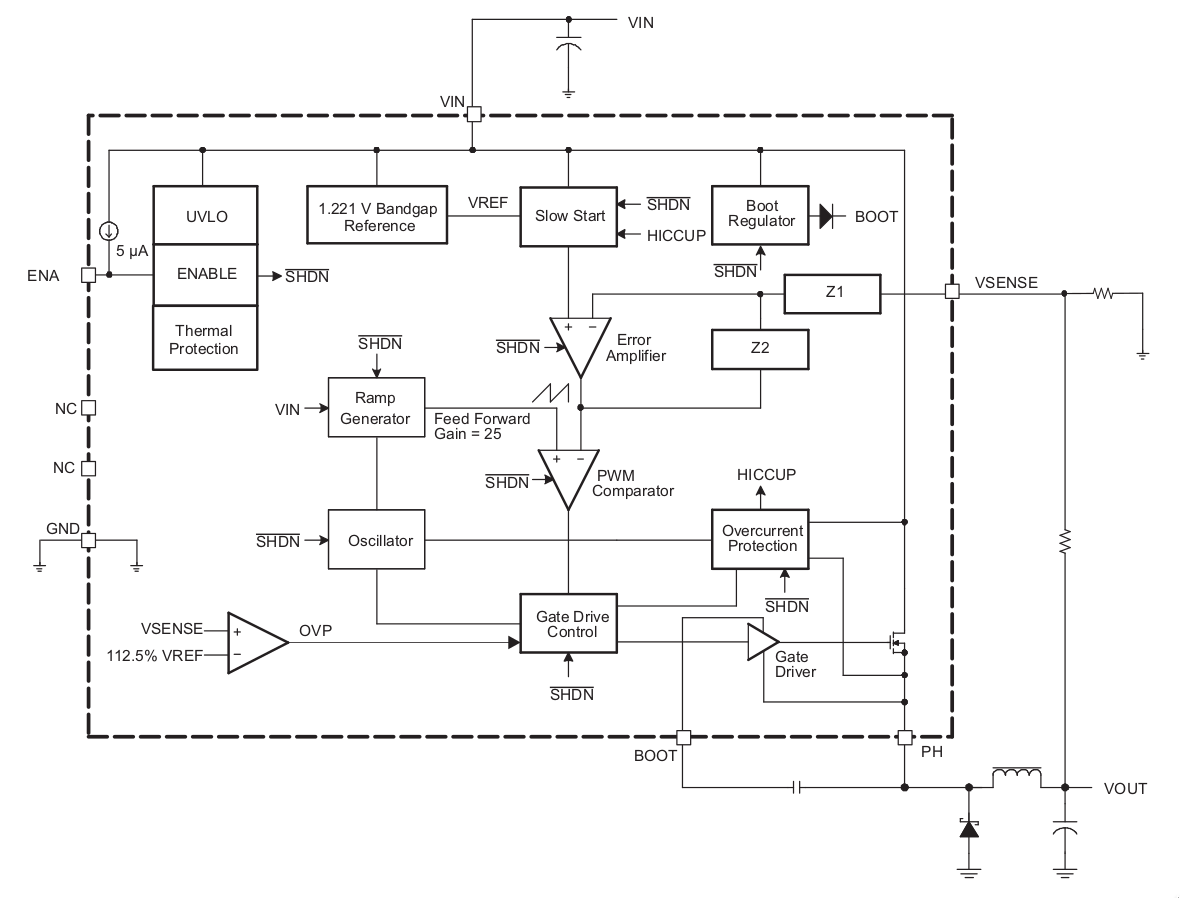
\includegraphics[width=0.9\textwidth]{data/tps5420d-block-diagram}
        \caption{TPS5420D Block Diagram}
        \label{fig:tps5420d-block}
\end{figure}

\subsubsection{Downstream Current Draw}

\label{tab:buck-5.6-downstream}
\begin{tabularx}{\textwidth}{l c c X>{\raggedright\arraybackslash}X}
        \caption{The current draw of components downstream from the 5.6V buck converter. Where the datasheet is
          ambiguous, I've assumed worst-case current draw.} \\
        \toprule
        \textbf{MFN} & \textbf{I\textsubscript{Q}} & \textbf{I\textsubscript{max}} & \textbf{Notes} \\
        \midrule
        \endhead
        \hyperlink{sec:adl5802}{ADL5802} & $170\si{mA}$ & $300\si{mA}$ & 5V \\
        \hyperlink{sec:adf4158}{ADF4158} & $312.5\si{\mu A}$ & $5\si{mA}$ & 5V (VP) \\
        \hyperlink{sec:se5004l}{SE5004L} & $300\si{mA}$ & $800\si{mA}$ & 5V (VCC1, VCC2, VCC3) \\
        \midrule
        Total & $470\si{mA}$ & $1.105\si{A}$ & - \\
        \bottomrule
\end{tabularx}

\label{tab:buck-3.6-downstream}
\begin{tabularx}{\textwidth}{l c c X>{\raggedright\arraybackslash}X}
        \caption{Components downstream from the 3.6V buck converter.} \\
        \toprule
        \textbf{MFN} & \textbf{I\textsubscript{Q}} & \textbf{I\textsubscript{max}} & \textbf{Notes} \\
        \midrule
        \endhead
        \hyperlink{sec:kt2520k}{KT2520K}  & - & $2\si{mA}$ & 1.8V \\
        \hyperlink{sec:nc7s04}{NC7S04} & $1\si{\mu A}$ & $12.5\si{mA}$ & 3.3V \\
        \hyperlink{sec:nb3n551}{NB3N551} & - & $40\si{mA}$ & 3.3V \\
        \midrule
        \hyperlink{sec:xc7a15t-ftg256}{XC7A15T-FTG256} & $97\si{mA}$ & $277\si{mA}$ & 1V (VCCINT, VCCBRAM) \\
        XC7A15T-FTG256 & $22\si{mA}$ & $87\si{mA}$ & 1.8V (VCCADC, VCCAUX) \\
        XC7A15T-FTG256 & $1\si{mA}$ & $201\si{mA}$ & 3.3V (VCC0) \\
        \hyperlink{sec:w25q32jv}{W25Q32JV} & $10\si{\mu A}$ & $25\si{mA}$ & 3.3V \\
        \midrule
        \hyperlink{sec:ft2232h}{FT2232H} & $510\si{\mu A}$ & $280\si{mA}$ & 3.3V (VPHY, VPLL, VCORE, VCCIO) \\
        \hyperlink{sec:93lc46b}{93LC46B} & - & $2\si{mA}$ & 3.3V \\
        \midrule
        \hyperlink{sec:ltc2292}{LTC2292} & $5\si{mA}$ & $95\si{mA}$ & 3.3V (OVDD), 3V (VDD) \\
        \midrule
        \hyperlink{sec:ada4940-2}{ADA4940-2} & $4.2\si{mA}$ & $5.52\si{mA}$ & 3.3V \\
        \midrule
        \hyperlink{sec:adf4158}{ADF4158} & - & $32\si{mA}$ & 3.3V (AVDD, DVDD) \\
        \midrule
        \hyperlink{sec:hmc431lp4}{HMC431LP4} & $19\si{mA}$ & $27\si{mA}$ & 3V \\
        \midrule
        \hyperlink{sec:trf37a73}{TRF37A73} & $250\si{\mu A}$ & $130\si{mA}$ & 3V \\
        \hyperlink{sec:sky65404}{SKY65404} & $20\si{mA}$ & $36\si{mA}$ & 3V (VENABLE, VCC) \\
        \midrule
        Total & $169\si{mA}$ & $1.252\si{A}$ & - \\
        \bottomrule
\end{tabularx}

\subsubsection{Pinout}
\label{sec:tps5420d-pinout}

\fixme{What is the point of BOOT?}
\label{tab:tps5420d-pinout}
\begin{tabularx}{\textwidth}{l X>{\raggedright\arraybackslash}X}
        \caption{TPS5420D pinout.} \\
        \toprule
        \textbf{Pin} & \textbf{Description} \\
        \midrule
        \endhead
        BOOT & \\
        VSENSE & Feedback voltage for the regulator. This compares the divided output with a 1.221V reference. \\
        ENA & Enable pin. This can be left floating to enable the device. \\
        VIN & Input supply voltage. \\
        PH & Output voltage. \\
        \bottomrule
\end{tabularx}

\subsubsection{Component Selection}
\label{sec:tps5420d-component-selection}

We will choose an inductor such that it satisfies the following 3 requirements:
\begin{enumerate}
\item The inductance is given by Equation~\ref{eq:buck-inductance}.
\item The current rating is 2x the maximum load current.
\item The self-resonant frequency is at least 10x the switching frequency.
\end{enumerate}

\begin{equation}
        \label{eq:buck-inductance}
        L_{\text{min}} = \frac{T}{2} \frac{V_{\text{out}}}{I_{\text{out(min)}}} \left(1 -
                \frac{V_{\text{out}}}{V_{\text{in}}}\right)
\end{equation}

The requirements are given in Table~\ref{tab:buck-inductor-reqs}. All of these requirements are satisfied by the
\href{https://www.bourns.com/docs/Product-Datasheets/SRR1210A.pdf}{SRR1210A-330M} $33\si{\mu H}$ ferrite bead by Bourns.

\label{tab:buck-inductor-reqs}
\begin{tabularx}{\textwidth}{c c c c}
        \caption{TPS5420D inductor requirements. I've assumed an input ripple of $300\si{mV}$.} \\
        \toprule
        \textbf{Buck Vout} & \textbf{Lmin} & \textbf{Current Rating} & \textbf{SRF min} \\
        \midrule
        \endhead
        $5.6\si{V}$ & $6.5\si{\mu H}$ & $2.21\si{A}$ & $5\si{MHz}$ \\
        $3.6\si{V}$ & $15.1\si{\mu H}$ & $2.50\si{A}$ & $5\si{MHz}$ \\
        \bottomrule
\end{tabularx}

\subsection{L7980 Buck Converter}
\label{sec:l7980-buck}

The L7980's block diagram is shown in Figure~\ref{fig:l7980-block-diagram} and its pin connections
are described in Table~\ref{tab:l7980-pins}.

\begin{figure}[h]
        \centering
        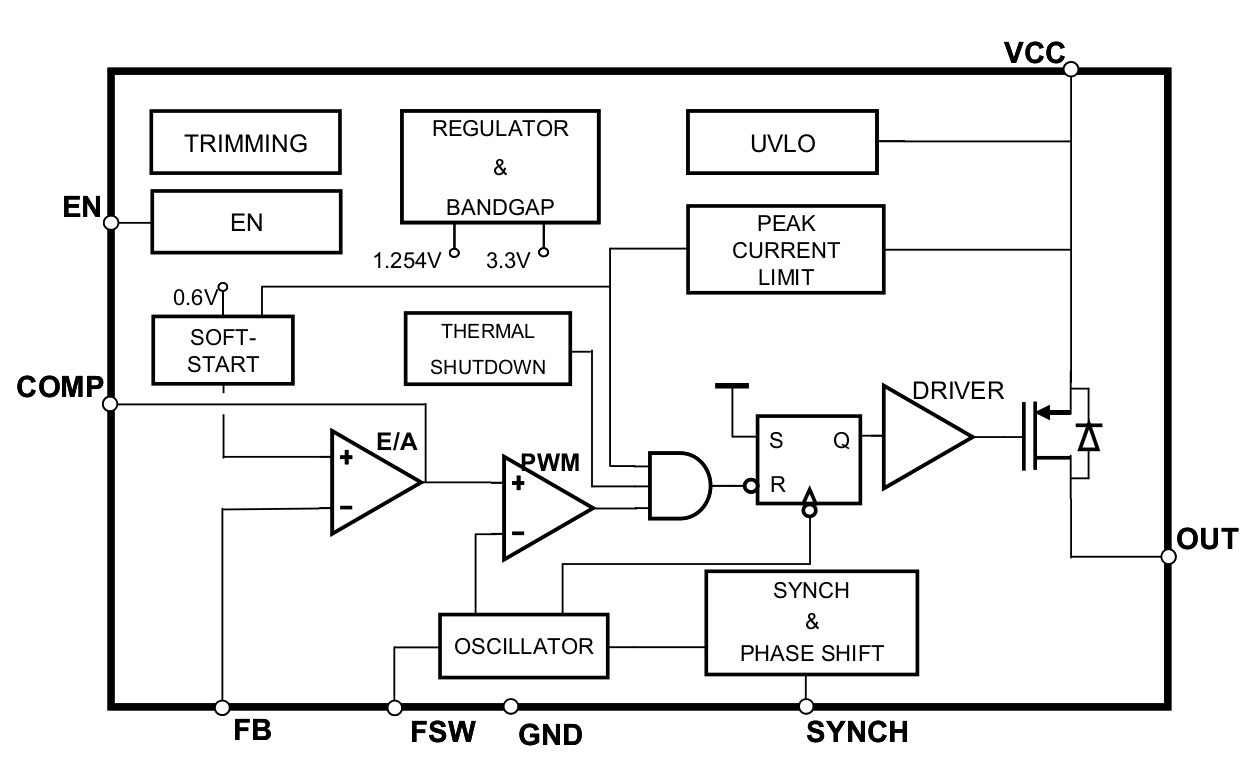
\includegraphics[width=0.75\textwidth]{data/l7980-block-diagram}
        \caption{L7980 buck converter block diagram.}
        \label{fig:l7980-block-diagram}
\end{figure}

\label{tab:l7980-pins}
\begin{tabularx}{\textwidth}{c X>{\raggedright\arraybackslash}X}
        \caption{L7980 pin connections.} \\
        \toprule
        \textbf{Pin} & \textbf{Description} \\
        \midrule
        \endhead

        OUT & Regulated output voltage. \\
        SYNCH & Synchronization pin that can be used when multiple L7980s are used on the same board. This
        pin serves a dual purpose: it allows an L7980 with a higher switching frequency (set with FSW) to
        synchronize an L7980 with a lower switching frequency and shifts its phase by half a period. That
        is, the ``master'' (the L7980 with a higher frequency) device makes its internal frequency
        available on this pin but phase shifted. Now, the lower frequency converters have that higher
        frequency at a phase shift. This reduces noise through destructive interference. This can also be
        used with an externally supplied frequency, but we don't do that here. \\
        EN & Active-high enable pin. \\
        COMP & The error amplifier output which is used for loop frequency compensation. More on this
        below. \\
        FB & The feedback input. This is fed into the inverting input of an error amplifier against a 0.6V
        reference. Therefore, we connect our output with a voltage divider to this pin such that it is
        0.6V when we have the desired output voltage. \\
        FSW & A resistor can be connected between this pin and ground to increase the converter's
        switching frequency. See Equation~\ref{eq:l7980-freq}. Leaving the pin free-floating sets the
        frequency at 250kHz, which is its minimum. \\
        GND & Ground. \\
        VCC & The unregulated DC input voltage. In our case, 12V from the barrel jack. \\

        \bottomrule
\end{tabularx}

The radar contains 3 L7980s that output 5.6V, 3.6V and 1V. The two higher voltages are fed to linear
regulators for further down-regulation and noise-filtering. The last is fed directly as one of the
input voltages to the FPGA.

\subsubsection{Switching Frequency}
\label{sec:l7980-switching-frequency}

The equation relating the resistor value at FSW to the switching frequency is:

\begin{equation}
        R_{\text{SW}}=\frac{28.5\times 10^9}{F_{\text{SW}}-250\times 10^3}-3.23\times 10^3
        \label{eq:l7980-freq}
\end{equation}

The 5.6V output buck converter uses a resistor of $59\si{k\ohm}$, which corresponds to a switching
frequency of 708kHz. This converter exports its internal frequency to the 3.6V output converter, so
although that converter uses a $68\si{k\ohm}$ resistor, it also switches at 708kHz. The 1V output
converter does not have its synchronization pin tied to the other two so its frequency (determined
by the $68\si{k\ohm}$ resistor) is 650kHz.

\subsubsection{Inductance Value}
\label{sec:l7980-inductance-value}

The benefit of a higher switching frequency is a lower minimum inductance value, which decreases the
cost of a circuit ($L_{\text{min}}\propto 1/F_{\text{SW}}$). To select an inductor value, we use
Equation~\ref{eq:L-select-eqn}.

\begin{equation}
        \Delta I_{\text{L}} = \frac{V_{\text{IN}}-V_{\text{OUT}}}{L} T_{\text{ON}}
        \label{eq:L-select-eqn}
\end{equation}

The duty cycle for buck converters is given by Equation~\ref{eq:duty-cycle}. Since
$V_{\text{IN}} = 12V$ and $V_{\text{OUT}} = 5.6V$, $D = 47\%$. We already found that the switching
frequency is 708kHz, which gives a total period of $1. 41\si{\mu s}$ and therefore
$T_{\text{ON}} = 0.659\si{\mu s}$. The inductor value used is $33\si{\mu H}$ which gives an inductor
current ripple of 128mA. This 5.6V output is used to power an ADL5802 mixer (\cref{sec:adl5802}),
which has a quiescent current of $220\si{mA}$. Since half the inductor ripple is less than the
mixer's minimum current draw, the inductor will stay in CCM and the mixer will see a stable output
voltage.

\begin{equation} DV_{\text{IN}} = V_{\text{OUT}}
        \label{eq:duty-cycle}
\end{equation}

\subsubsection{PWM}
\label{sec:l7980-pwm}

This device uses a voltage-mode PWM comparator to stabilize the output voltage at its desired
level. The block diagram shows how this works. The divided output voltage is fed back into the
inverting input of the error amplifier and a 0.6V reference is fed to the non-inverting input. The
error amplifier's output is compared against a sawtooth waveform at the inverting input, generated
by the built-in oscillator. As long as the error amplifier voltage is greater than that of the
sawtooth waveform the flip-flop reset is not triggered and the PMOS transistor is switched
on. However, once the sawtooth waveform voltage becomes greater than that of the error amplifier,
the active-low reset will be triggered on the flip-flop and the transistor will switch off until the
next clock pulse from the internal oscillator. So, when the output voltage goes above its intended
level the duty cycle decreases and when it goes below its intended level the duty cycle increases.

\subsubsection{Loop Compensation}
\label{sec:l7980-loop-compensation}

The COMP pin is used to provide feedback to the error amplifier, which in turn generates the error
voltage signal that is compared with the internal sawtooth signal to determine the pulse modulation
that controls the voltage output. There are two different compensation networks that we can use, as
described in the datasheet: type II compensation and type III compensation. The datasheet recommends
the use of type III compensation for MLCC capacitors given their low ESR. \textbf{\{START
  INCOMPLETE\}} The actual calculation of these values is tricky and requires knowledge of feedback
and op-amps, which in turn requires prerequisite knowledge of transistors. I believe it's probably
necessary to complete chapters 1-4 of the Art of Electronics to understand this, so I intend to come
back to it. On the upside, this should provide a solid background for DSP \textbf{\{END
  INCOMPLETE\}}.

The buck converter outputs feed into several different chips, the first of which is an LDO regulator
for which an example is shown in Figure~\ref{fig:linear-reg}. The reason for attaching an LDO
regulator in series with a buck converter may be to reduce the noise of the circuit and increase the
efficiency at the expense of board area and cost. Particularly, the
\href{http://www.ti.com/lit/ds/symlink/tps7a91.pdf}{LDO regulator} should be able to smooth out the
noise caused by using an inductor with a low value in the buck converter. It is meant to effectively
reject noise from the input source over the frequency range of 10Hz to 10MHz. Since the switching
frequency of the buck converter is less than 1MHz and consequently the current/voltage ripple should
be of the same frequency, the LDO regulator should be sufficient to smooth out the input noise
provided, however, that it does not dip below the output voltage of the LDO regulator since the
margin for error is small. $V_{\text{IN}}-V_{\text{OUT}}=0.6V$ and linear regulators are not able to
output a voltage greater than their input voltage. The max dropout of the LDO is 0.2V, which allows
the output voltage of the buck converter a deviation of 0.4V.

\begin{figure}[h]
        \centering
        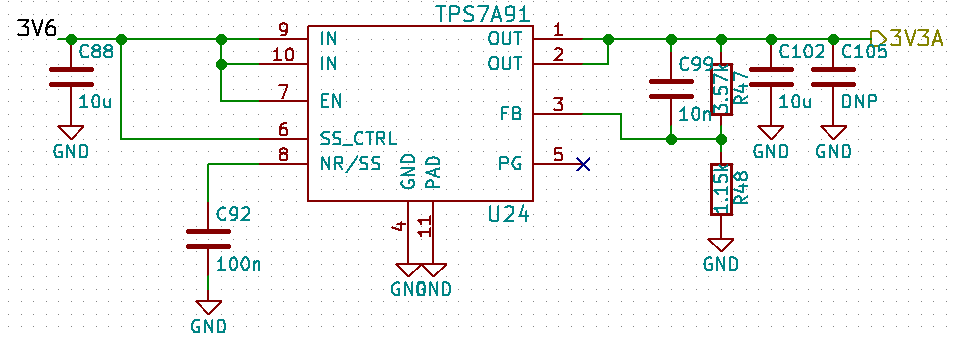
\includegraphics[width=0.75\textwidth]{data/linear-reg.png}
        \caption{A LDO regulator that takes as an input the voltage from one of the buck converters and
          whose output is directly used to drive the operation of one of the ICs elsewhere in the
          circuit.}
        \label{fig:linear-reg}
\end{figure}

The input voltage is connected to both IN pins with a bypass capacitor of 10 $\mu$F, which is the
minimum specified by the datasheet. It is additionally connected to the EN pin which activates the
LDO; the LDO is active for $V_{\text{EN}} \geq V_{\text{IH}}$ and disabled for
$V_{\text{EN}} \leq V_{\text{IL}}$ (connecting the same input to IN and EN will make
$V_{\text{EN}} = V_{\text{IH}}$, thus satisfying the first condition). The 2 resistors attached to
OUT and FB make a voltage divider that determines the output voltage of the linear regulator,
according to Equation~\ref{eq:linear-reg-vout}.

\begin{equation}
        R_1 = R_2\left(\frac{V_{\text{OUT}}}{V_{\text{REF}}}-1\right) \label{eq:linear-reg-vout}
\end{equation}

Where $V_{\text{REF}} = 0.8V$ Specifically, 1.15k and 3.57k are specified in the datasheet in order
to get an output voltage of 3.3V. SS\_CTRL is connected to IN instead of GND which increases the
soft-startup charging current to 100 $\mu$A from 6.2 $\mu$A and decreases the start-up time, which
is given by Equation~\ref{eq:linear-reg-startup-time}.

\begin{align}
  t_{\text{SS}} &= (V_{\text{REF}} \times C_{\text{NR/SS}}) /
                  I_{\text{NR/SS}} \label{eq:linear-reg-startup-time} \\
                &= 0.8V \times 100 \times 10^{-9} F/(100 \times 10^{-6} A) \\
                &= 0.8\text{ms}
\end{align}

An output capacitor of 10 $\mu$F is chosen which is the minimum specified by the
datasheet. Additionally, a feed-forward capacitor of 10nF is added between the OUT and FB pins to
improve the noise and PSRR performance of the voltage regulator. The value is recommended by the
datasheet. The $C_{\text{NR/SS}}$ capacitor of 100nF is used to create an output RC filter for
output noise and is also used to set the soft-start time. A value of between 10nF and 10$\mu$F is
recommended. PAD and GND should both be connected to ground, as indicated by the datasheet. PG
indicates whether the output voltage is in a usable state. Since we are not using it, it can be left
floating.

Another buck converter output feeds into the input of an ultra low LDO, with a dropout voltage of
40mV as shown in Figure~\ref{fig:ldo-ldo-connection}. R104 acts as a pull-up resistor, pulling the
voltage on EN high when PG is not driven. However, when PG is low, EN will be driven low. The bypass
pin is left open, although a 1$\mu$F capacitor could have been placed there to reduce output noise.

\begin{figure}[h]
        \centering
        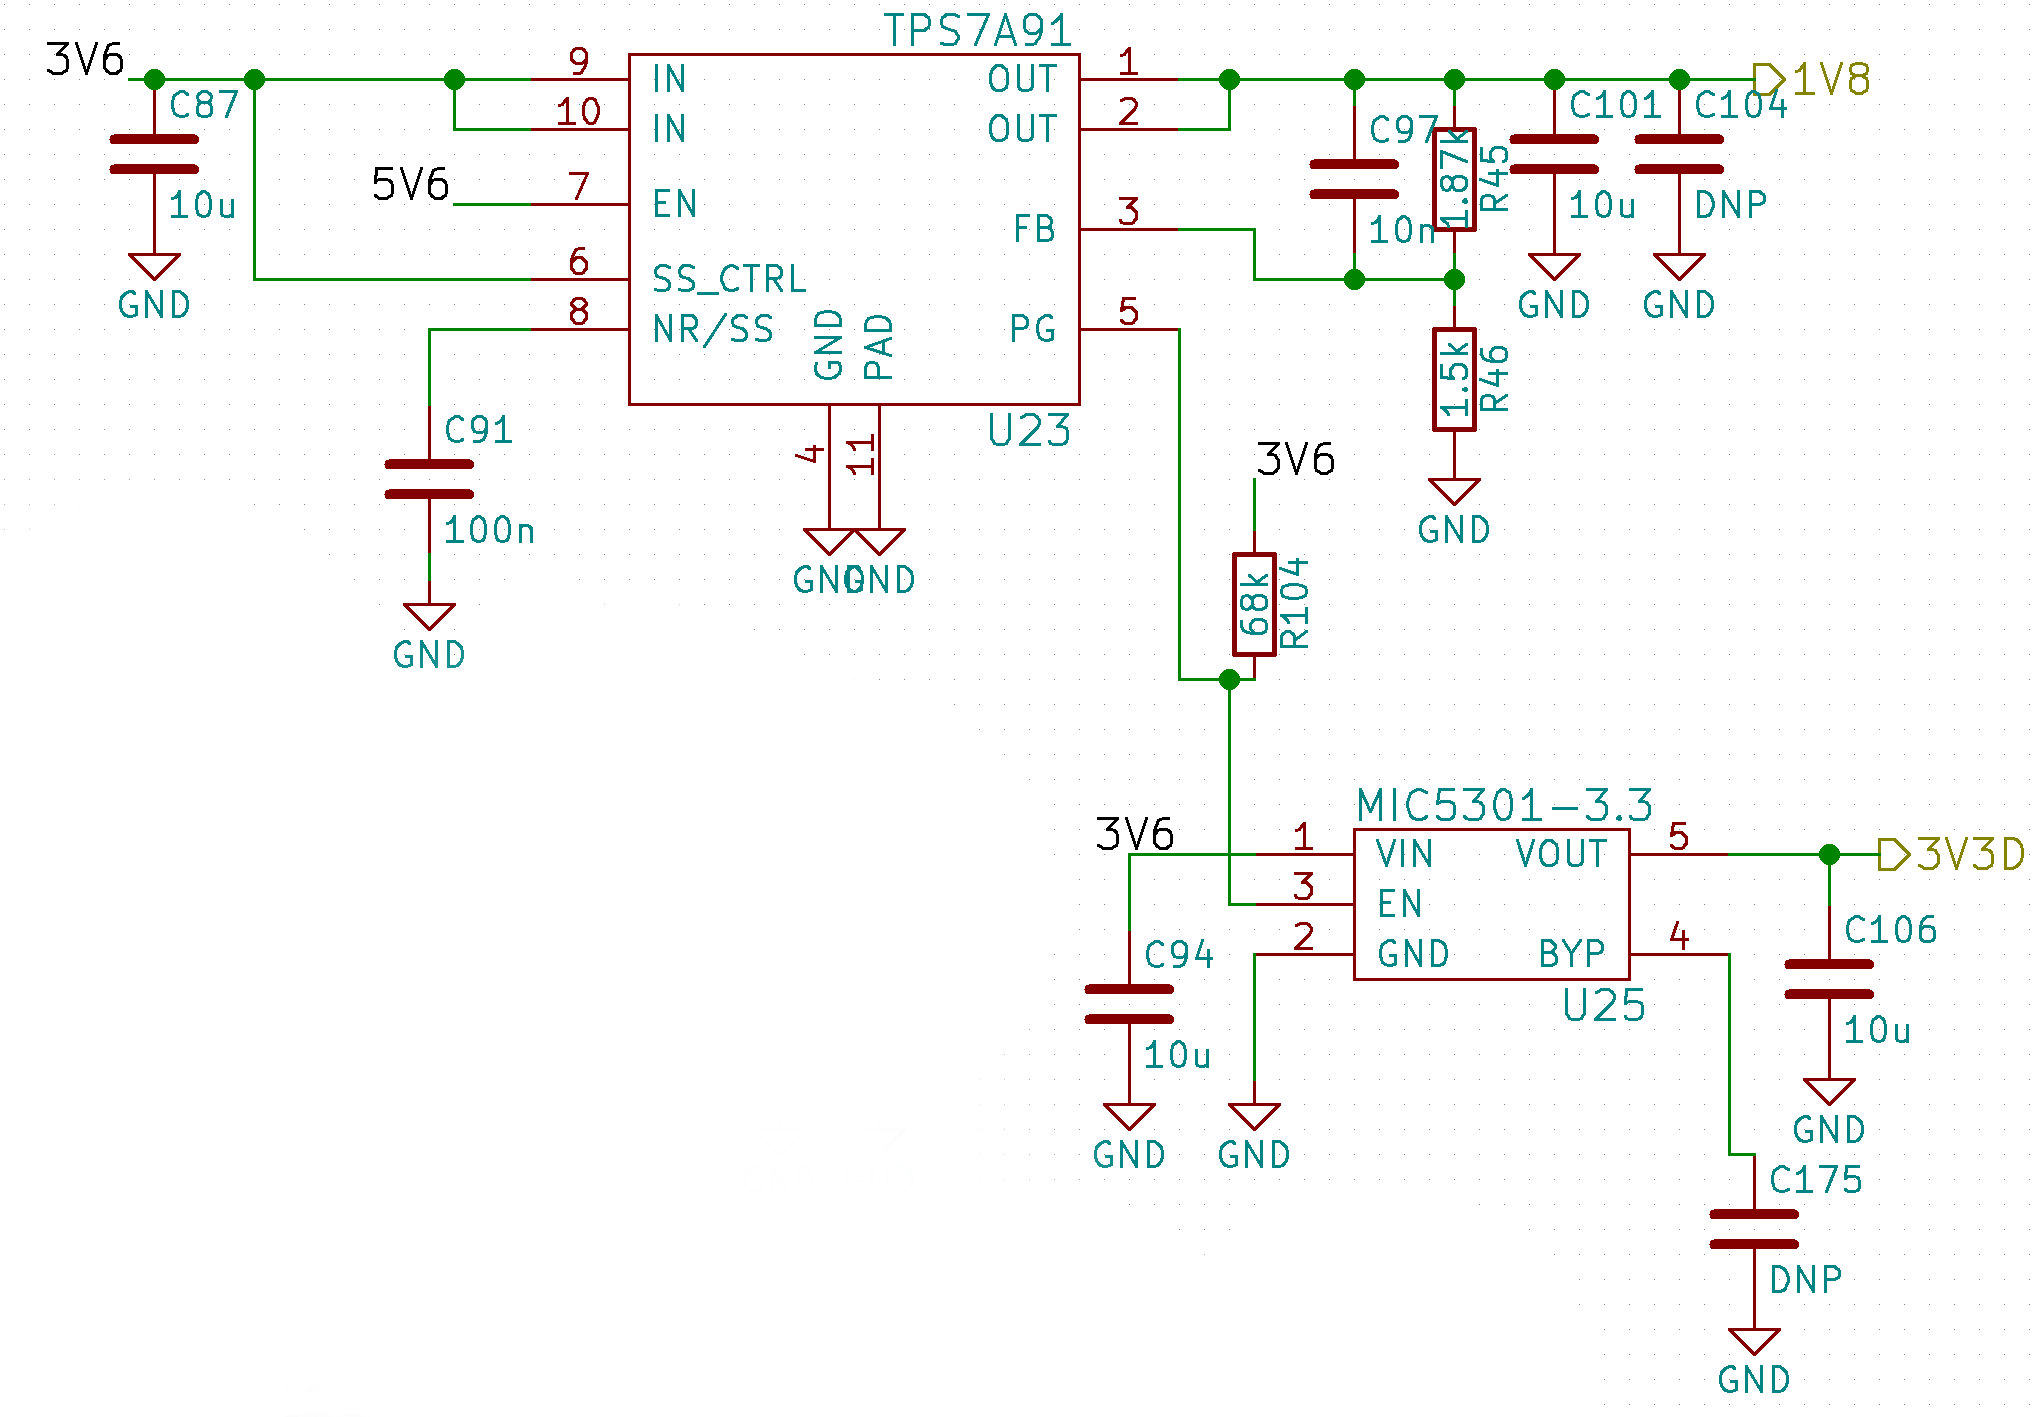
\includegraphics[width=0.9\textwidth]{data/ldo-ldo-connection.png}
        \caption{An ultra LDO regulator whose output feeds into an FPGA input. It uses the PG
          pin from another LDO regulator to alternately enable/disable it.}
        \label{fig:ldo-ldo-connection}
\end{figure}

Another output from a buck converter leads to a 3V output LDO regulator with a dropout voltage of
120mV shown in Figure~\ref{fig:lp5907}. All of the pin connections are evident.

\begin{figure}[h]
        \centering
        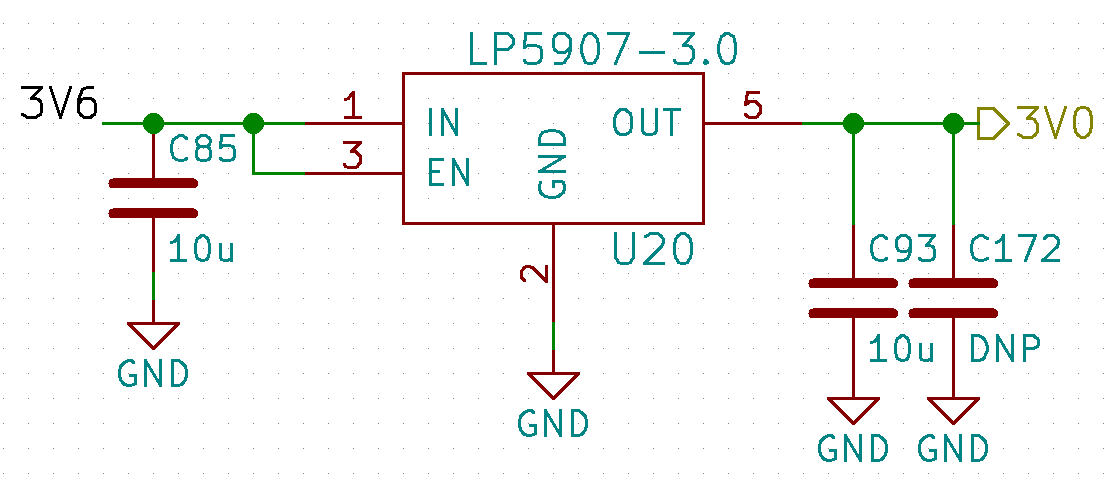
\includegraphics[width=0.75\textwidth]{data/lp5907.png}
        \caption{The LP5907 is a 3V LDO regulator with a dropout voltage of 120mV.}
        \label{fig:lp5907}
\end{figure}

The last component on the power sheet is an
\href{http://www.ti.com/lit/ds/symlink/lp2985.pdf}{LP2985} LDO regulator shown in
Figure~\ref{fig:lp2985}, that takes the 12V input voltage from the barrel jack and outputs
10V. ON/OFF is an active-low shutdown pin, so it is tied to $V_{\text{IN}}$. A 10nF capacitor is
tied to BYPASS to decrease the output noise.

\begin{figure}[h]
        \centering
        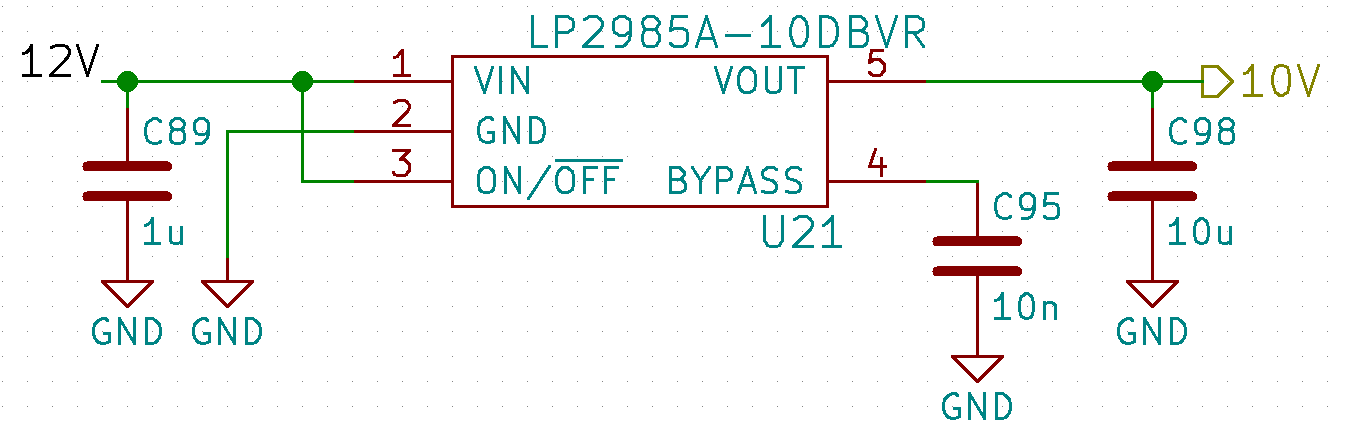
\includegraphics[width=0.9\textwidth]{data/lp2985.png}
        \caption{The LP2985 LDO regulator.}
        \label{fig:lp2985}
\end{figure}